\section{Simulation}

\subsection{Robot wingman}

\begin{frame}{A robot Wingman problem}{Robot Wingman}

\begin{figure}
\centering
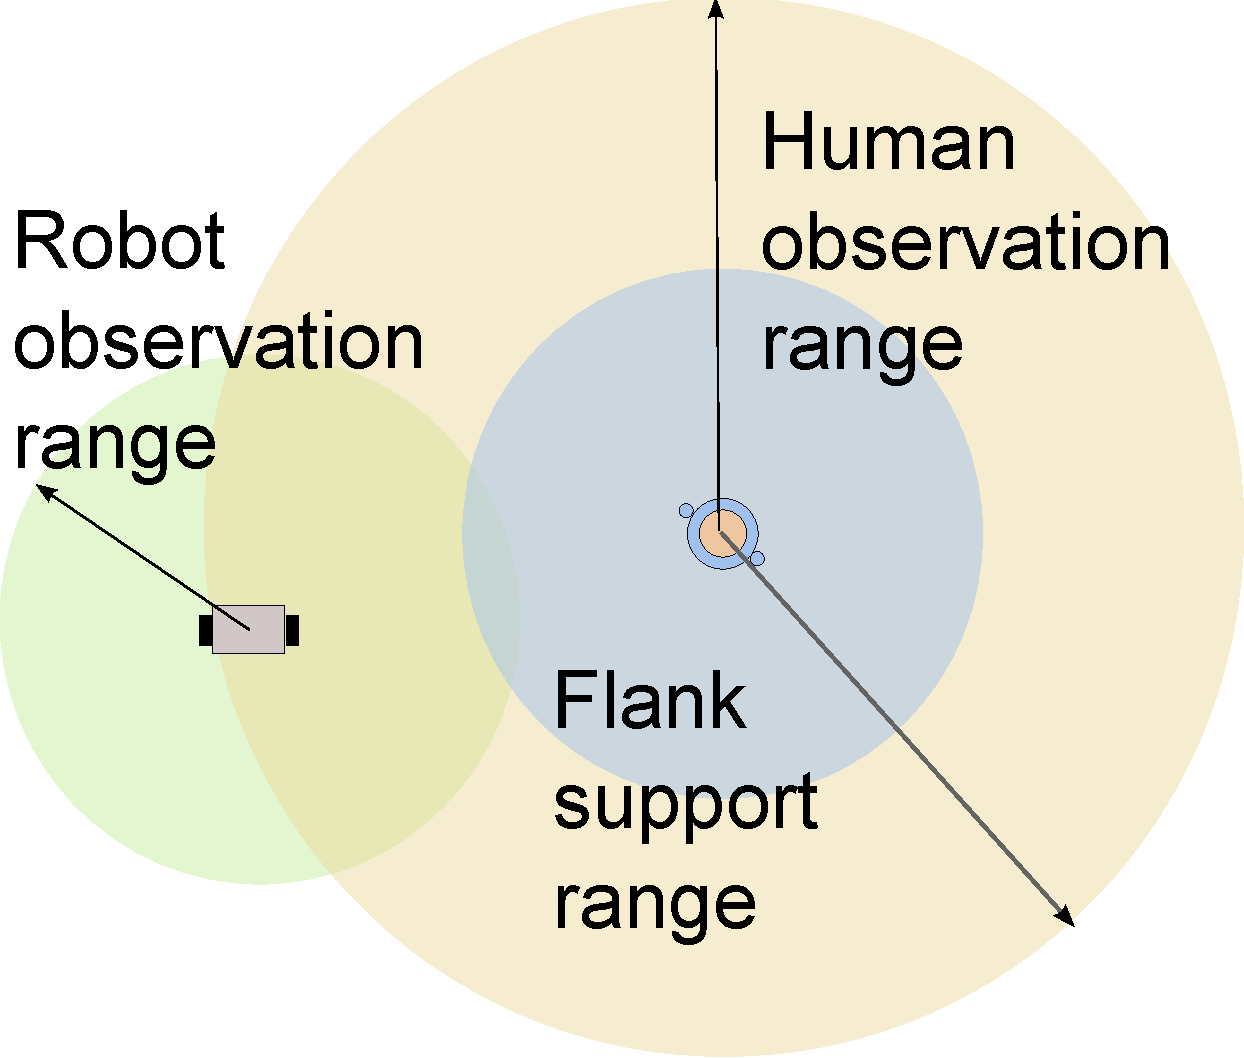
\includegraphics[width = 0.6\textwidth]{./figure/Wingman}
\end{figure}

\end{frame}

\begin{frame}{Labelling}{Robot wingman}

%\begin{minipage}
\begin{columns}
\column{0.25\textwidth}

\column{0.4\textwidth}
\begin{minipage}{\textwidth}
\begin{block}{Gazebo world}
\centering
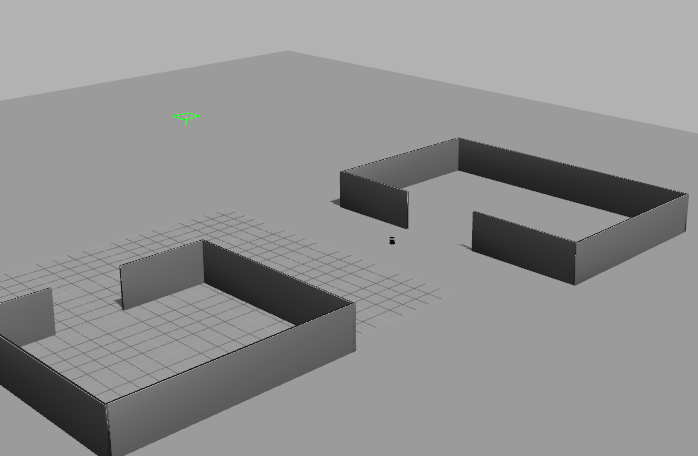
\includegraphics[width = \textwidth]{./figure/simulation/gazebo.png}
\end{block}
\end{minipage}

\column{0.1\textwidth}
\begin{minipage}{\textwidth}
\centering

\includegraphics[width = \textwidth]{./figure/arrow2}
\end{minipage}

\column{0.25\textwidth}
\end{columns}

%\bigskip

\begin{columns}

\column{0.1\textwidth}

\column{0.275\textwidth}
\begin{minipage}{\textwidth}
\begin{block}{Map}
\centering
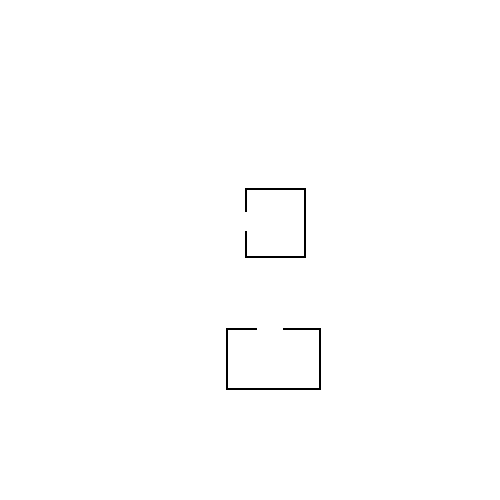
\includegraphics[width = \textwidth]{./figure/simulation/map.png}
\end{block}
\end{minipage}

\column{0.1\textwidth}
\begin{minipage}{\textwidth}
\centering

\includegraphics[width = \textwidth]{./figure/arrow2}
\end{minipage}

\column{0.275\textwidth}
\begin{minipage}{\textwidth}
\begin{block}{Labeling}
\centering
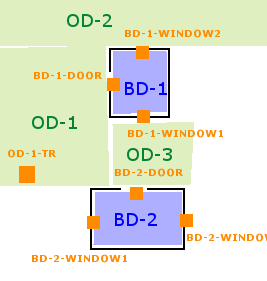
\includegraphics[width = \textwidth]{./figure/simulation/label.png}
\end{block}
\end{minipage}

\column{0.1\textwidth}

\end{columns}
%\end{minipage}

\end{frame}

\begin{frame}{Path planning}{Robot wingman}

\begin{columns}
\column{0.05\textwidth}

\column{0.275\textwidth}
\begin{minipage}{\textwidth}
\begin{block}{Path planning}
\centering
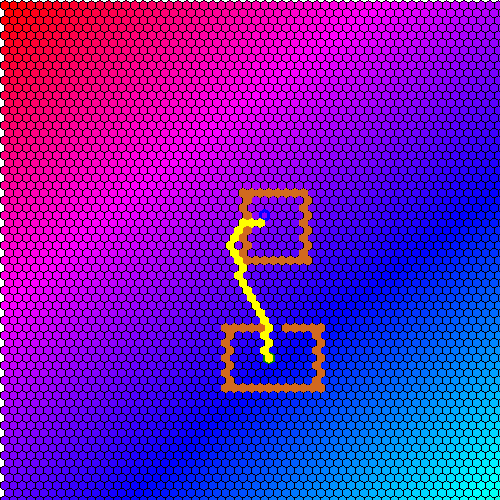
\includegraphics[width = \textwidth]{./figure/simulation/hexamap.png}
\end{block}
\end{minipage}

\column{0.2\textwidth}
\begin{minipage}{\textwidth}
\centering

\includegraphics[width = 0.5\textwidth]{./figure/arrow2}
\end{minipage}

\column{0.275\textwidth}
\begin{minipage}{\textwidth}
\begin{block}{Waypoints}
\centering
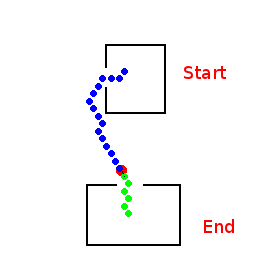
\includegraphics[width = \textwidth]{./figure/simulation/waypoint.png}
\end{block}
\end{minipage}

\column{0.05\textwidth}
\end{columns}

%\bigskip

\begin{columns}
\column{0.25\textwidth}

\column{0.1\textwidth}
\begin{minipage}{\textwidth}
\centering

\includegraphics[width = \textwidth]{./figure/arrow2}
\end{minipage}

\column{0.4\textwidth}
\begin{minipage}{\textwidth}
\begin{block}{Robot execution}
\centering
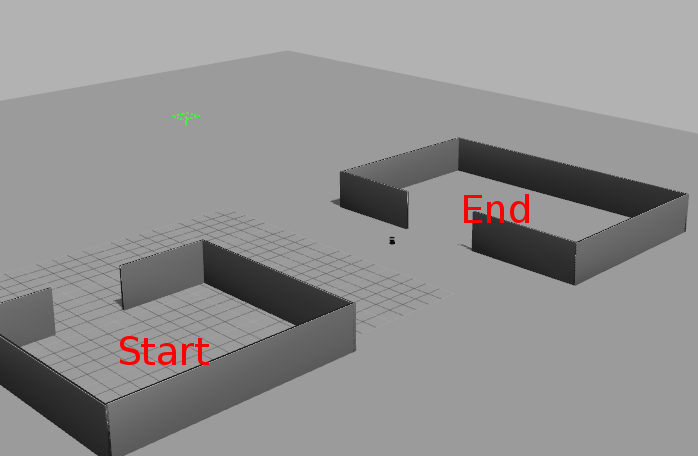
\includegraphics[width = \textwidth]{./figure/simulation/gazebo2.png}
\end{block}
\end{minipage}

\column{0.25\textwidth}

\end{columns}

\end{frame}

\subsection{Results}

\begin{frame}{Metrics}{Results}

\begin{itemize}
\item \textcolor{metric-PR}{\textbf{Problem size}} \\
nodeNum(\dashuline{fully expanding tree}) 

\item \textcolor{metric-NE}{\textbf{Percentage of nodes explored}}
%\textcolor{green}{[efficiency]}
\\
nodeNum(\dashuline{current expanding tree}) / nodeNum(\dashuline{fully expanding tree})

\item \textcolor{metric-OFI}{\textbf{Percentage of optimal at first iteration}}
%\textcolor{red}{[goodness]}
\\
score(\dashuline{first found solution}) / score(\dashuline{optimal solution})

\item \textcolor{metric-IRO}{\textbf{Number of iterations to reach optimal (normalized)}}
%\textcolor{red}{[goodness]}
\\
iterationCount(\dashuline{optimal found}) / iterationCount(\dashuline{finish tree expanding})
\end{itemize}

\end{frame}

\begin{frame}

quality of heuristic


quality of algorithm

\end{frame}

\begin{frame}{Performance}{Results}

\begin{columns}
\column{0.45\textwidth}
\begin{minipage}{\textwidth}
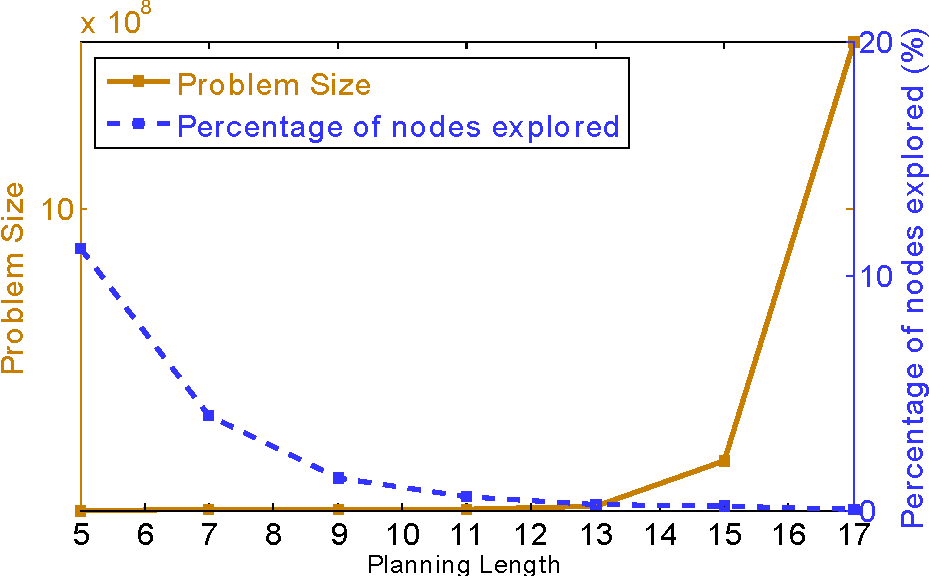
\includegraphics[width=\textwidth]{./figure/T_ProbSize_ExpRatio}
\end{minipage}
\column{0.45\textwidth}
\begin{minipage}{\textwidth}
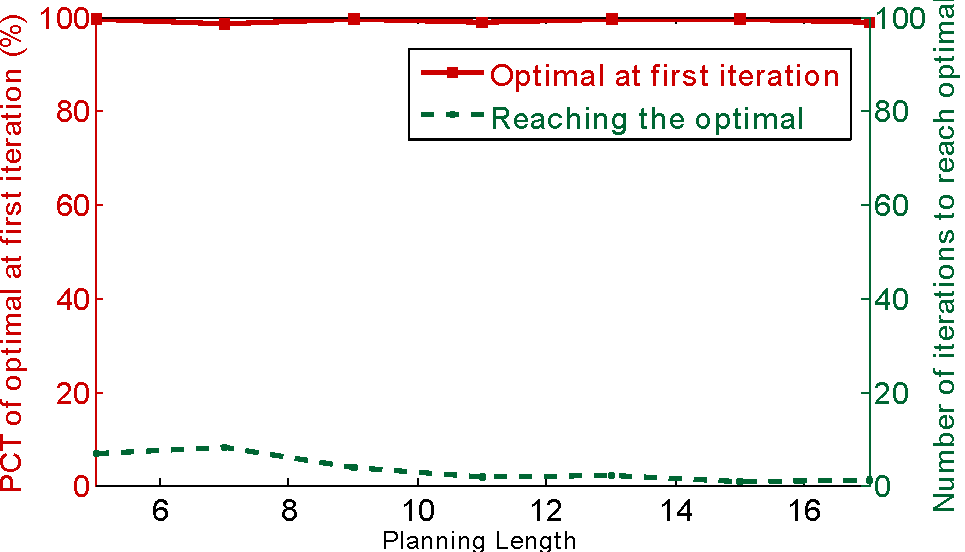
\includegraphics[width=\textwidth]{./figure/T_InitOpt_OptRch}
\end{minipage}
\end{columns}

\end{frame}

\begin{frame}{Compare with greedy heuristic}{Performance}

The performance of the heuristic (Percentage of optimal at first run)

\bigskip
\bigskip

%\begin{columns}
%\column{0.45\textwidth}
%\begin{minipage}{\textwidth}
%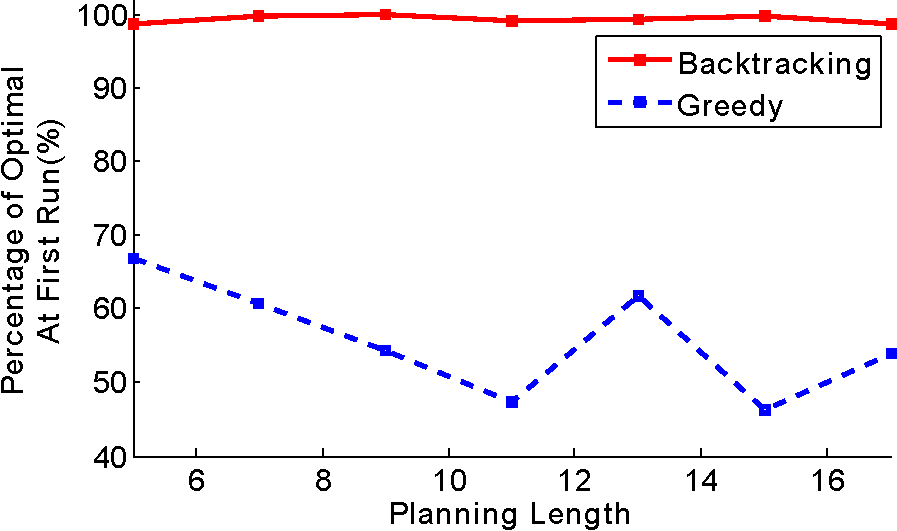
\includegraphics[width=\textwidth]{./figure/compareGreedy}
%\end{minipage}
%\column{0.45\textwidth}
%\begin{minipage}{\textwidth}
%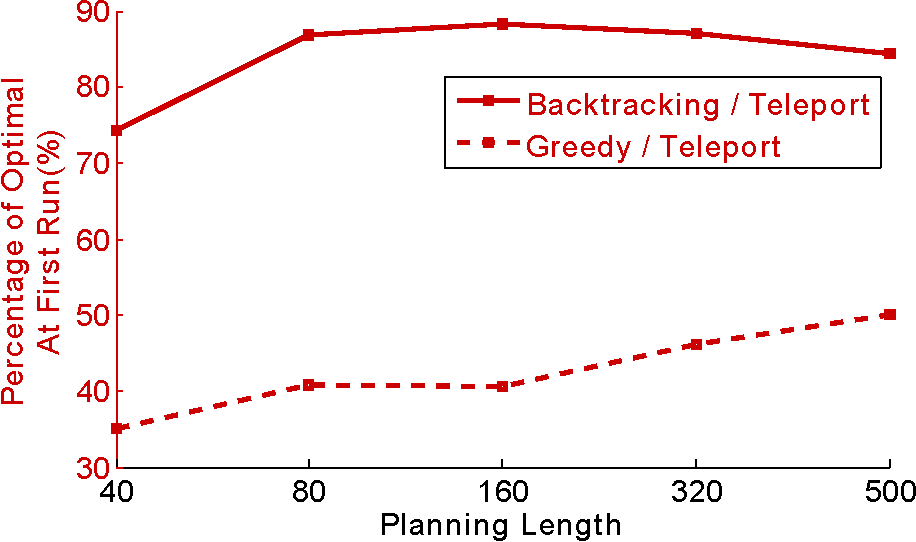
\includegraphics[width=\textwidth]{./figure/largeprob}
%\end{minipage}
%\end{columns}

\begin{figure}
\centering
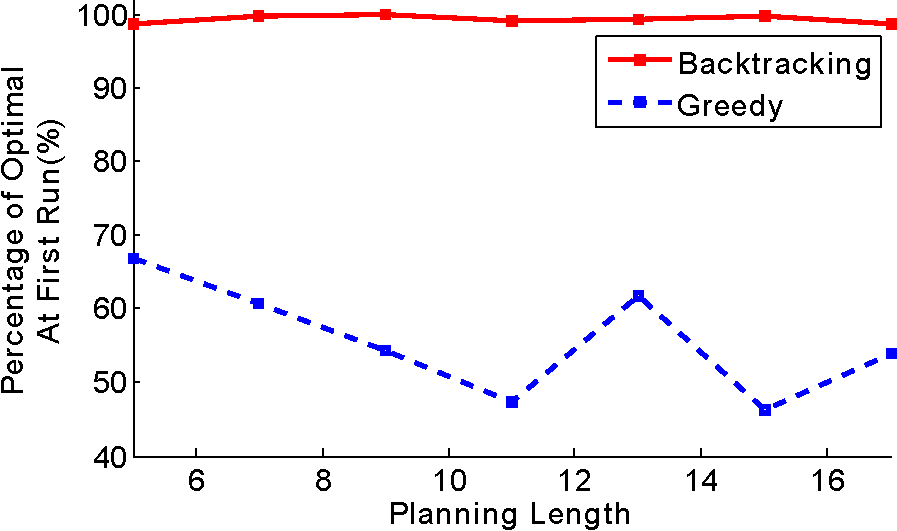
\includegraphics[width=0.6\textwidth]{./figure/compareGreedy}
\end{figure}

\end{frame}

\begin{frame}{Information pattern difference}{Robustness}

\begin{columns}

\column{0.22\textwidth}
\begin{block}{Uniform}
\begin{center}
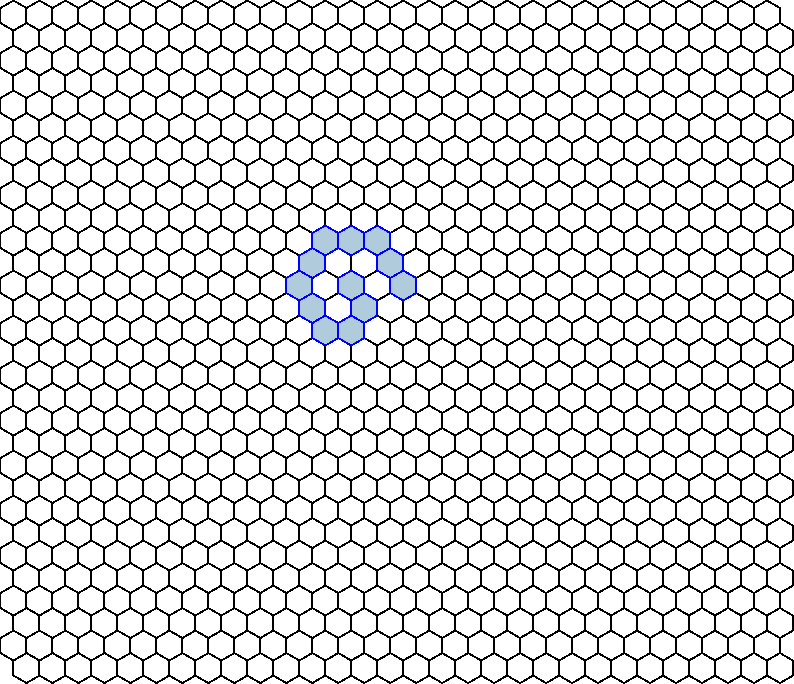
\includegraphics[width=0.8\textwidth]{./figure/ENV_UNI}
\end{center}
\end{block}
\column{0.22\textwidth}
\begin{block}{Random}
\begin{center}
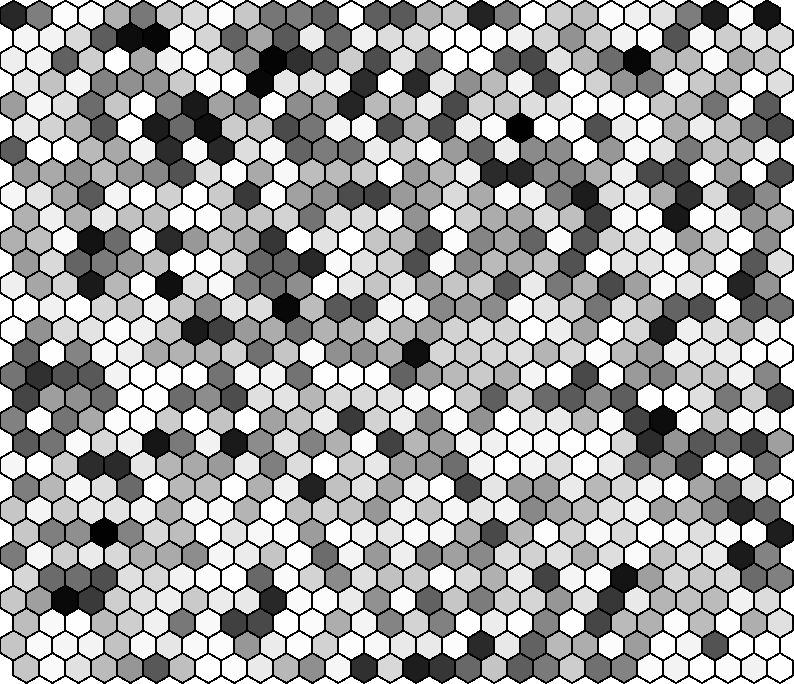
\includegraphics[width=0.8\textwidth]{./figure/ENV_RND}
\end{center}
\end{block}
\column{0.22\textwidth}
\begin{block}{Multi-Modal}
\begin{center}
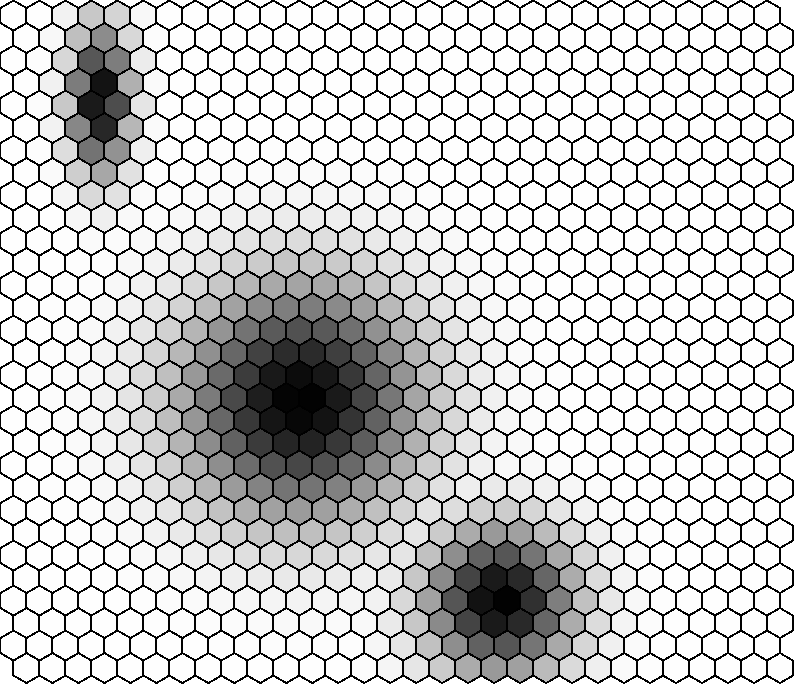
\includegraphics[width=0.8\textwidth]{./figure/ENV_MM}
\end{center}
\end{block}

\end{columns}

\begin{center}
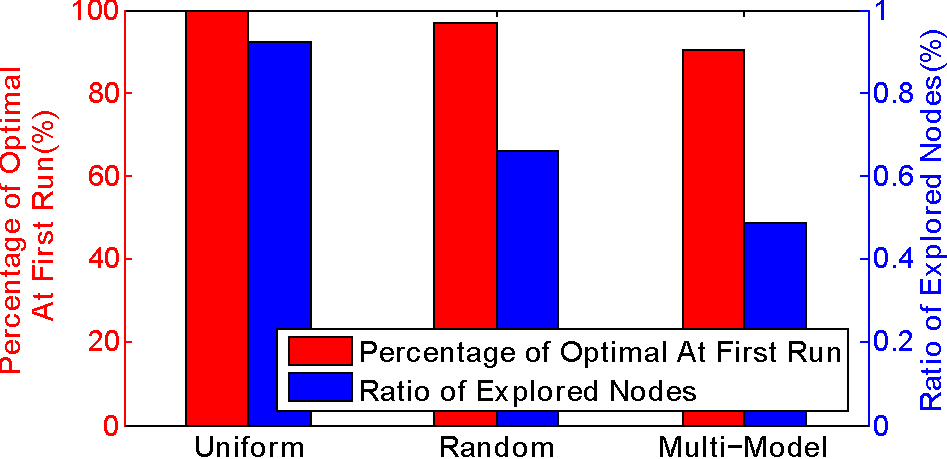
\includegraphics[width=0.6\textwidth]{./figure/EnvPerform}
\end{center}


\end{frame}

\begin{frame}{Human path difference}{Robustness}

\begin{columns}[T]
\column{.3\linewidth}
\begin{block}{Line}
\begin{minipage}[c][.2\textheight][c]{\linewidth}
\begin{figure}
\centering
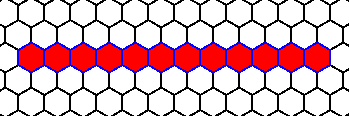
\includegraphics[width = 0.8\textwidth]{./figure/HMP_Line_Small.png}
\end{figure}
\end{minipage}
\end{block}

\column{.3\linewidth}
\begin{block}{Spiral}
\begin{minipage}[c][.2\textheight][c]{\linewidth}
\begin{figure}
\centering
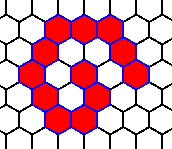
\includegraphics[width = 0.4\textwidth]{./figure/HMP_Spiral_Small.png}
\end{figure}
\end{minipage}
\end{block}

\column{.3\linewidth}
\begin{block}{Lawn mower}
\begin{minipage}[c][.2\textheight][c]{\linewidth}
\begin{figure}
\centering
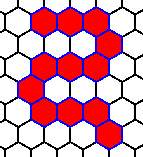
\includegraphics[width = 0.33\textwidth]{./figure/HMP_LawnMower_Small.png}
\end{figure}
\end{minipage}
\end{block}
\end{columns}

\bigskip

\begin{columns}[T]
\column{.3\linewidth}
\begin{block}{Arc}
\begin{minipage}[c][.2\textheight][c]{\linewidth}
\begin{figure}
\centering
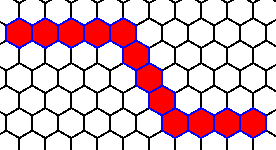
\includegraphics[width = 0.7\textwidth]{./figure/HMP_Arc_Small.png}
\end{figure}
\end{minipage}
\end{block}

\column{.3\linewidth}
\begin{block}{Loitering}
\begin{minipage}[c][.2\textheight][c]{\linewidth}
\begin{figure}
\centering
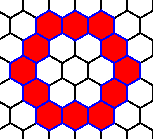
\includegraphics[width = 0.4\textwidth]{./figure/HMP_Loitering_Small.png}
\end{figure}
\end{minipage}
\end{block}
\end{columns}

\end{frame}

\begin{frame}{Human path difference}{Robustness}

\begin{columns}

\column{0.4\textwidth}
\begin{minipage}{\textwidth}
%\begin{center}
%Problem size
%\end{center}
\begin{figure}
\centering
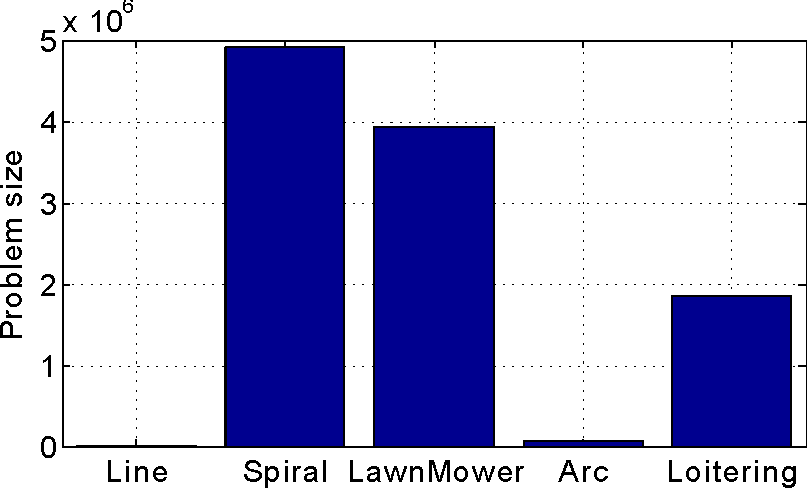
\includegraphics[width=\textwidth]{./figure/ProbSizeInDiffHMP}
\end{figure}
\end{minipage}

\column{0.4\textwidth}
\begin{minipage}{\textwidth}
%\begin{center}
%Ratio of explored nodes
%\end{center}
\begin{figure}
\centering
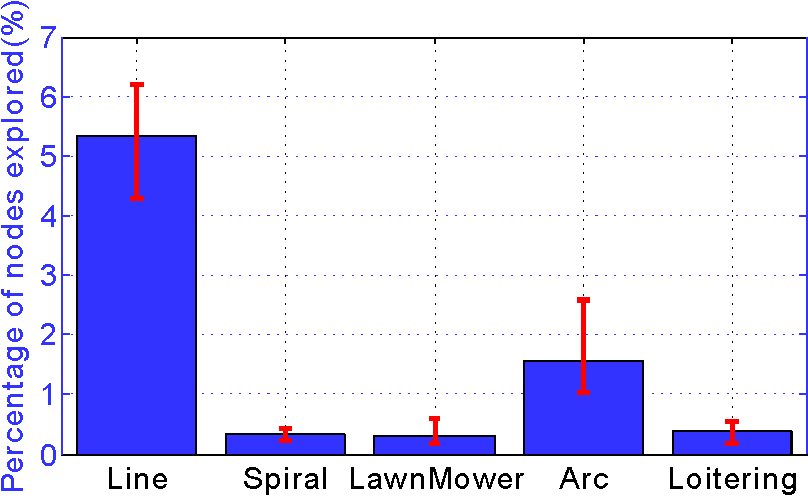
\includegraphics[width=\textwidth]{./figure/ExpRatioInDiffHMP}
\end{figure}
\end{minipage}
\end{columns}

\bigskip

\begin{columns}
\column{0.6\textwidth}
\begin{minipage}{\textwidth}
%\begin{center}
%Percentage of optimal at first run
%\end{center}
\begin{figure}
\centering
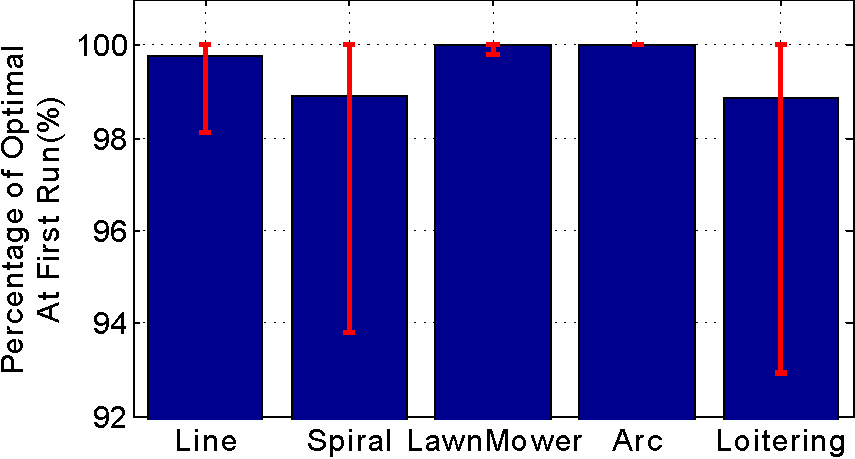
\includegraphics[width=0.7\textwidth]{./figure/InitOptInDiffHMP}
\end{figure}
\end{minipage}
\end{columns}

\end{frame}